\documentclass[12pt,a4paper,oneside]{article}

\usepackage[spanish]{babel}

\def\mydate{\leavevmode\hbox{\the\year-\twodigits\month-\twodigits\day}}
\def\twodigits#1{\ifnum#1<10 0\fi\the#1}

\usepackage{fancyhdr}
\usepackage{geometry}
\usepackage{graphicx}
\usepackage{wrapfig}
\usepackage{lastpage}
\usepackage[hidelinks]{hyperref}
\usepackage{authblk}
\usepackage{bookmark}

\usepackage[utf8]{inputenc} % Required for inputting international characters
\usepackage[T1]{fontenc} % Output font encoding for international characters
\usepackage{mathpazo} % Palatino font

\makeatletter
\newcommand{\subtitledoc}[1]{\newcommand{\@subtitledoc}{#1}}
\newcommand{\instituto}[1]{\newcommand{\@instituto}{#1}}
\newcommand{\carrera}[1]{\newcommand{\@carrera}{#1}}
\newcommand{\professor}[1]{\newcommand{\@professor}{#1}}
\newcommand{\catedra}[1]{\newcommand{\@catedra}{#1}}
\newcommand{\curso}[1]{\newcommand{\@curso}{#1}}
\newcommand{\legajo}[1]{\newcommand{\@legajo}{#1}}
\newcommand{\footerauthor}[1]{\newcommand{\@footerauthor}{#1}}
\newcommand{\footerlegajo}[1]{\newcommand{\@footerlegajo}{#1}}
\newcommand{\footercatedra}[1]{\newcommand{\@footercatedra}{#1}}

%Configuracion de hoja (margenes y tamaño)
\geometry{a4paper,margin=1in}
\setlength\headheight{28pt}

%Metadata para pdf
%\hypersetup{
%    pdftitle={\@title},
%    pdfsubject={\@catedra\ - \@subtitledoc},
%    pdfauthor={\@author\ - \@legajo\ - \@curso},
%    pdfkeywords={\@title\ \@catedra\ \@subtitledoc\ \@author\ \@legajo\ \@curso}
%}

%formato de encabezado y pie para todas las paginas.
\fancyhead[L]{
  \begin{minipage}[b]{7.5mm}
    
\includegraphics[width=7mm]{imagenes/COPYlogo-utn.eps}
  \end{minipage}
  \begin{minipage}[b]{85mm}
    \textbf{Alumnos: }\@footerauthor\\
    \textbf{Legajos: }\@footerlegajo
  \end{minipage}
}
\fancyhead[R]{
  %\textbf{Comisión:} \@curso 
  \textbf{Fecha:} \mydate \\
  \textbf{Cátedra:} \@footercatedra \text{ (}\@curso\text{)}
}
\fancyfoot[C]{} %eliminar antiguo numero de pagina
\fancyfoot[R]{Página \thepage\ de \pageref{LastPage}}
\renewcommand{\headrulewidth}{0.5pt}
\renewcommand{\footrulewidth}{0.5pt}
\pagestyle{fancy}

\addto\captionsspanish{%
  \renewcommand{\contentsname}%
  {CONTENIDO}%
}

\renewcommand{\maketitle}{%
  \newpage
  \thispagestyle{empty}

  \begin{center}

    \textsc{\LARGE \@instituto}\par
    \vspace{0.5cm}
    \textsc{\Large \@carrera}\par
    \vspace{1cm}
    
\includegraphics[width=0.30\textwidth]{imagenes/COPYlogo-utn.eps}\par
    \vspace{1cm}

    \textsc{\Large \@catedra}\par
    \vspace{1.5cm}

    \hrule
    \vspace{0.5cm}
    {\huge\bfseries \@title}\par
    \vspace{0.4cm}
    \textsc{\large \@subtitledoc}
    \vspace{0.5cm}
    \hrule \vspace{\baselineskip}


  \end{center}

  \vspace{2cm}

  {\noindent
    \begin{minipage}[t]{.2\textwidth}
      \raggedright
      \textbf{DOCENTES} \par
      \vspace{\baselineskip}
      %\textbf{CÁTEDRA} \par
      \medskip
      \medskip
      \textbf{COMISIÓN} \par
      \medskip
      \medskip
      \textbf{ALUMNOS} \par
    \end{minipage}%
    \begin{minipage}[t]{.05\textwidth}
      \raggedright
      %\textbf{:} \par
      %~\\
      %~\\
      %\textbf{:} \par
      %\textbf{:} \par
      %\medskip
      %\medskip
      %\textbf{:} \par
    \end{minipage}%
    \begin{minipage}[t]{.55\textwidth}
      \raggedright
      \@professor. \par
      \medskip
      %\@catedra. \par
      \medskip
      \@curso \par
      \medskip
      \medskip
      \@author 
    \end{minipage}%
    \begin{minipage}[t]{.15\textwidth}
      \raggedright
      \vspace{\baselineskip}
      \vspace{\baselineskip}
      \medskip
      \bigskip
      % \medskip
      \medskip
      \medskip
      \@legajo \par
    \end{minipage}
  }
  \vfill
  \begin{center}
    {\Large\textbf{Córdoba, \@date}} \vspace{\baselineskip}
    %\medskip
    %\textbf{Córdoba, Argentina} \par
    \newpage
  \end{center}
}

\makeatother

\usepackage{listings}
\usepackage{amsmath}
\usepackage[section]{placeins}
\usepackage{subfig}
\usepackage[nottoc,numbib]{tocbibind}
\usepackage{titlesec}
\usepackage{xcolor}
\definecolor{codegreen}{rgb}{0,0.6,0}

\definecolor{codegray}{rgb}{0.5,0.5,0.5}
\definecolor{codepurple}{rgb}{0.58,0,0.82}
\definecolor{backcolour}{rgb}{0.95,0.95,0.92}

\lstdefinestyle{mystyle}{
  backgroundcolor=\color{backcolour},   
  commentstyle=\color{codegreen},
  keywordstyle=\color{magenta},
  numberstyle=\tiny\color{codegray},
  stringstyle=\color{codepurple},
  basicstyle=\ttfamily\footnotesize,
  breakatwhitespace=false,         
  breaklines=true,                 
  captionpos=b,                    
  keepspaces=true,                 
  numbers=left,                    
  numbersep=5pt,                  
  showspaces=false,                
  showstringspaces=false,
  showtabs=false,                  
  tabsize=2
}

\lstset{style=mystyle}

\setcounter{secnumdepth}{4}

\titleformat{\paragraph}
{\normalfont\normalsize\bfseries}{\theparagraph}{1em}{}
\titlespacing*{\paragraph}
{0pt}{3.25ex plus 1ex minus .2ex}{1.5ex plus .2ex}

\instituto{Universidad Tecnológica Nacional\\Facultad Regional Córdoba}
\carrera{Ingeniería Electrónica}
\title{Brazo Robótico tri axial}
\subtitledoc{Trabajo Práctico Grupo N°2}
\catedra{Informática II}
\professor{Herencia Juan José,\\ Martinez José Luis}
\curso{2R2}
\author{De Robles Agustin\par Giorgis Ezequiel\par Luna Joaquín}
\legajo{80499\\91661\\ 75934}
\footerauthor{De Robles, Giorgis, Luna}
\footerlegajo{80499, 91661, 72934}
\footercatedra{Informática II}
\date{\today}

\begin{document} %Maximo 10 paginas
\maketitle
\tableofcontents
\newpage

\section{Resumen} % Max 200 palabras
\section{Introducción} % 1 a 2 paginas
  El presente documento tiene como fin exponer, desarrollar y explicar la codificación realizada en la construcción de un brazo robótico triaxial.
Para la elección del tema nos inspiramos en las lineas de producción y en su constante desarrollo e importancia. Particularmente en los brazos robóticos que, por una cuestión de reducción de costos y mayor eficacia en su trabajo, están cada vez mas presentes en las fabricas.
\par
Nuestro objetivo fue construir un brazo robótico que pueda recibir instrucciones por computadora con la finalidad de moverse en tres ejes y abrir y cerrar una pinza con presicion. En un futuro tambien podría adaptase para categorizar un producto según su color, su forma o tamaño. 

  \subsection{Descripción general} % Fotos del equipo
    \input{descripciónGral.tex}
\section{Hardware} % Diagrama de bloques?
En el apartado de hardware se destaca, como bien dijimos, el uso de tres 
motores paso a paso 28BYJ-48 cuyas especificaciones son:
\begin{itemize}
  \item Tensión nominal de entre 5V y 12 V.
  \item 4 Fases.
  \item Resistencia 50 Ω.
  \item Par motor de 34 Newton / metro (aprox. 0,34 Kg por cm).
  \item Consumo de unos 55 mA.
  \item 8 pasos por vuelta.
  \item Reductora de 1 / 64.
  \item Unipolar
\end{itemize}
\begin{figure}[!htb]
  \begin{center}
    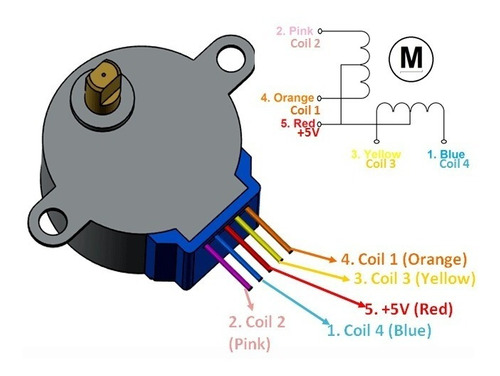
\includegraphics[width=0.4\textwidth]{imagenes/28BYJ_48.jpg}
  \end{center}
  \caption{Motor $28BYJ_48$}
  \label{fig:28BYJ_48}
\end{figure}
\FloatBarrier
Para controlar estos motores, se emplearón drives UNL2003 constituido por dos transistores en configuración Darlington.
\begin{figure}[!htb]
  \begin{center}
    \subfloat[]{{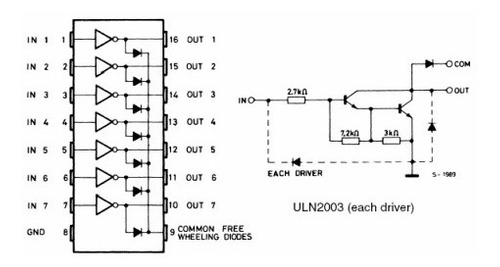
\includegraphics[width=6cm]{imagenes/ULN2003.jpg} }}%
    \qquad
    \subfloat[]{{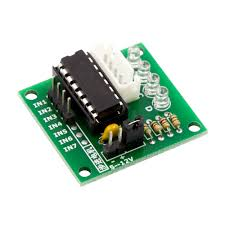
\includegraphics[width=4cm]{imagenes/ULN2003_PCB.jpg} }}%
  \end{center}
  \caption{Driver ULN2003}
  \label{fig:Driver ULN2003}
\end{figure}
\FloatBarrier
Para la apertura y cierre de la pinza, se utilizó un servo motor Sg90; el cual posee
un torque de 9 gramos.
\begin{figure}[!htb]
  \begin{center}
    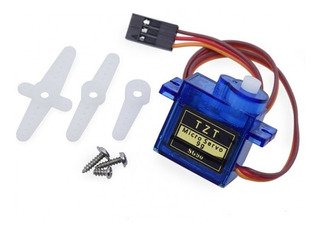
\includegraphics[width=0.4\textwidth]{imagenes/servo.jpg}
  \end{center}
  \caption{Servo Sg90}
  \label{fig:servo}
\end{figure}



\section{Proceso de compilado y flash}
 Para la compilación del código correspondiente al microcontrolador,
 como así también al de la PC, se emplearon los siguientes compiladores y programas/utilidades
 de consola:
 \begin{itemize}
   \item gcc 
   \item g++ 
   \item avr-dude 
   \item avr-copy
   \item avr-size
 \end{itemize}
 Todos ellos implementados en la herramienta de gestión de dependencias Make.


\section{Software Microcontrolador}
\subsection{Función Main}
Dentro del código se incluyen todos los archivos de cabecera dentro de un único llamado allInc.h. 
Este último contiene, entre otras cosas, las funciones SetInOut, pwm init y las relacionadas a la Uart.
\par
Con las funciones SetInOut se inicializan los pines del arduino, con UART init 
se configura la velocidad para la uart y la comunicación serial y con pwm init 
se inicializa el pwm y se setea el valor mínimo $(0)$ y máximo $(180)$ del 
servomotor para la amplitud de la apertura de la pinza.
En el bucle infinito, la función UART gets lee el puerto de serie hasta que 
haya un salto de línea, almacenando el dato en la variable line para luego 
traducirlo con la función parse en comandos de movimiento, devolviendo error u 
ok según corresponda.


\lstinputlisting[language=c]{../software/micro/src/main.c}
\subsection{UART}\label{UART}
Debido a las necesidades del presente proyecto, se optó por la utilización de una comunicación en serie asíncrona de tipo half-duplex bajo el estándar RS-232 con una configuración de trama 115200/8N1. Las características de dicha comunicación entre dispositivos se detallan a continuación:
\par
\paragraph*{Comunicación serie}
    La comunicación serie o serial transmite un único bit a la vez de forma secuencial, es decir, un bit tras otro, uno a la vez. Aunque es más lenta que una comunicación paralela, tiene la ventaja de que físicamente requiere de una sola conexión (un solo cable). Además, tiene un límite de distancia mucho mayor frente a una comunicación en paralelo.
    \par
    \paragraph*{Asíncrona}
En la comunicación asíncrona, la sincronización se restablece con la transmisión de cada carácter mediante el uso de bits de inicio y parada que, dependiendo de la tecnología utilizada, puede haber 1, 1,5 o 2 bits de parada.
\par
\paragraph*{Half-Duplex}
 De manera similar, cuando dos dispositivos de comunicación de datos se comunican en un entorno Half-Duplex, un dispositivo debe ser el transmisor y el otro el receptor. Para permitir la comunicación bidireccional, periódicamente tienen que invertir roles.    
 \par
 \paragraph*{Estándar RS-232}
La sección de características eléctricas del estándar RS-232 incluye especificaciones sobre los niveles de tensión, tasa de cambio de niveles de las señales e impedancia de la línea. El estándar RS-232 original se definió en 1962, previo a los días de la lógica TTL (Transistor-Transistor Logic), por lo que no es de extrañar que no utilice niveles lógicos de 5 voltios. En cambio, se define un nivel alto de salida con tensiones entre +5 y +15 voltios y un nivel bajo entre –5 y –15 voltios. Los niveles lógicos de entrada se definieron para proporcionar un margen de ruido de 2 voltios, por lo tanto un nivel alto para la entrada debe estar comprendido entre +3 a +15 voltios y un nivel bajo entre –3 a –15 voltios. En el actual proyecto, por incidencia directa del microcontrolador Atmega328, se emplearon salidas de +5V para niveles lógicos altos. 
\par
\paragraph*{Velocidad de transmisión}
    Indica el número de bits por segundo. En nuestro caso 115200 por defecto.
    \paragraph*{Trama 8n1}
    \par
    \paragraph*{El número de bits de datos}
    Refiere a la cantidad de bits (word) en la transmisión. En nuestro caso 8 bits.
    \par
    \paragraph*{El número de bits de stop}
    Utilizado para indicar el fin de la comunicación de un paquete. Mientras más bits de paro se usen, mayor será la tolerancia a la sincronía de los relojes de los dispositivos involucrados, sin embargo, la transmisión será más lenta. Para este proyecto se utilizó un bit de stop.
    \par
    \paragraph*{Y si cuenta con bit de paridad}
    El bit de paridad es una forma sencilla de verificar si hay errores en la transmisión serial. Para nuestro contexto no fue necesario definir bits de paridad, puesto que la complejidad de los datos enviados y recibidos no era elevada.
    \par
Finalmente para configurar, con las características mencionadas con anterioridad, la UART del microcontrolador Atmega328  se modificaron los registros correspondientes según la hoja de datos del fabricante y según la siguiente fórmula para determinar el registro de UART Baud Rate Register (UBRR0).
\begin{figure}[!htb]
  \begin{center}
    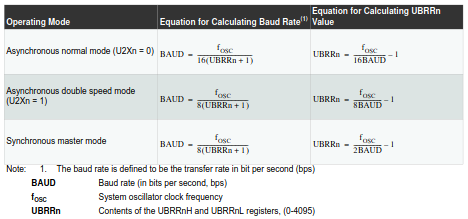
\includegraphics[width=0.92\textwidth]{imagenes/UARTbaudRateTable.png}
  \end{center}
  \caption{Tabla para calcular el registro de Baud Rate}
  \label{fig:baudRateTable}
\end{figure}
\FloatBarrier


\lstinputlisting[language=c, firstline=3, lastline=17]{../software/micro/src/UART_utils.c}
\subsection{Funciones parse y execLine}
Nos permite ingresar una cadena de caracteres en donde discrimina los espacios en blanco. Posteriormente mediante la función strToUpper nos permite hacer la conversión a una letra Mayúscula. Esto nos permite mayor tolerancia al momento de ingresar en qué eje se ha de desplazar el brazo, tomando en cuenta que si se ingresa una letra Minúscula hará la conversión correspondiente y permitirá realizar la acción de los motores paso a paso. En dado caso en que se ingrese un carácter S ejecutará la acción de la función execLine que hará accionar el servo.
\par
Dado el caso en el que se ingrese x,y,z por teclado y también se ingrese un valor por ejemplo 100, la letra indicará hacia que eje debe hacer el movimiento el brazo y el valor indicará la cantidad de paso(step) que debe hacer en dicha dirección.
\par
El programa contempla el sentido en que debe desplazarse el brazo, dado que puede realizar el desplazamiento en ambos sentidos.

\subsection{Control de motores y servo motores}
Para conseguir esta secuencia se define, primeramente, un arreglo de tipo uint8 t (unsigned char) constante donde serán almacenados los pines y el puerto correspondiente a cada entrada del driver
Estos serán pasados, junto al número de pasos a ejecutar, por referencia y copia respectivamente, a la función moveAxisRelative. Esta define un contador para indicar el paso actual, por lo que varía entre 0 y 3. Por último, se hace uso de un arreglo de funciones, doStepHorario, para llamar a la función del paso que corresponda. Función que es la encargada de apagar y energizar las bobinas del motor por medio del registro de 8 bits correspondiente al puerto, y con el uso de los operadores a nivel de bit y sentencias correspondientes para apagar y encender respectivamente.
\par
Para la apertura y cierre del servomotor, se hizo uso de los timers del propio Atmega328 para generar una señal de pulso modulado (pwm). De este modo, 
haciendo variar el duty cycle de la señal, conseguimos que el servo motor se posición según lo deseado. 


\lstinputlisting[language=c, firstline=5, lastline=9]{../software/micro/src/stepper.c}
\section{Software PC}
\subsection{Comunicación serial}
Para llevar a cabo una comunicación serial exitosa, ambos dispositivos deben tener la misma configuración. Por ello, para implementar la configuración descrita en la sección (\ref{UART}) se abrió el dispositivo tratado como archivo, para luego settear sus características por medio de la estructura términos.

\lstinputlisting[language=c, firstline=38, lastline=49]{../software/pc/src/ttyConfig.c}
\subsection{Función Main}
Luego de abrir como un archivo y configurar el microcontrolador, se inicia un ciclo for infinito que 
permitirá enviar las correspondientes instrucciones al brazo: direcciones y sentido en las que se desee 
que se realice el desplazamiento como así también la cantidad de pasos (step) que deben hacer en dicha dirección.
Todo esto últimos datos son enviados en forma de cadena de caracteres al microcontrolador.

\lstinputlisting[language=c, firstline=48, lastline=58]{../software/pc/src/COPYmain.c}
\subsection{GUI}
El entorno gráfico cuenta con 13 botones en total, 12 para mover el brazo en los ejes x,y,z; y uno para accionar la pinza.
\par
En el código se inicializa el id del producto y el del proveedor del arduino uno. Se procede a reconocer los puertos disponibles y comparar el identificador del producto y el del proveedor conectados con los previamente seteados. Si coinciden, en la variable arduino uno port name se copia la información referente al puerto de serie, que se utilizará luego para inicializar el nombre del puerto. 
\par
Se procede a verificar que, dentro de la comunicación serial, el baudrate, los bits, la paridad, etc. sean los requeridos para seguir con el proceso. Se espera por un dato de entrada, dicha información se lee y se depura. En caso de no poder hacerlo se imprime un error. 
\par
Al presionar un botón, ejemplo -x se verifica que se pueda escribir el puerto de serie y, si es así, se envía un valor, en este caso, de -100.
\begin{figure}[!htb]
  \begin{center}
    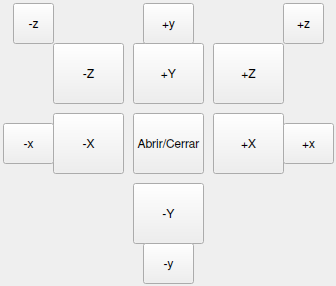
\includegraphics[width=0.5\textwidth]{imagenes/GUIscreenShot.png}
  \end{center}
  \caption{Implementación interfaz gráfica}
  \label{fig:GUI}
\end{figure}
\FloatBarrier


%\lstinputlisting[language=c]{../software/pc/src/main.c}
\section{Conclusiones}
La construcción final del brazo robótico demuestra de por sí la capacidad 
del quienes subscriben de programar softwares de bajo nivel necesarios para las industrias de hoy en 
día. Además, gracias al paradigma de programación estructurada por el que se opto, se logro
crear un código, no solo flexible, sino también reutilizable y adaptable según
la envergadura y necesidades de cada proceso industrial. 

\nocite{atmega328Datasheet}
\nocite{bjarneC++}
\nocite{deitel}
\nocite{make}
\nocite{CProgramingMicro}
\nocite{ControlPerifericosPaina}
\bibliography{inc/bibliografia}{}
\bibliographystyle{plain}

\end{document}
